% Chapter 15 (English edition) -- ED-24: independent rebuild, kernel replay and audit of the openai/NavierStokesAndEuler corpus
% Translated from papers/discovery_journal_2026/chapters/c15.tex. Figure: code/fig15.py.
\chapter[Rebuilding someone else's machine]{Rebuilding someone else's machine in your own workshop}

\reference{Published on 26 October 2026. doi:10.5281/zenodo.23661381}

\section*{The idea in one picture}

The Navier--Stokes equations describe how fluids flow, from water in a pipe to air around a wing.
The Clay Institute has made one question about them one of its ``Millennium Problems'': do smooth
solutions always exist, or can they ``break''? Its official description offers four possible
statements; two of them assert a breakdown.

In 2026, OpenAI published a set of Lean files, called here \emph{the corpus}, whose authors
present the content as the formalisation of two of these breakdown statements, plus a singularity
for the Euler equations, another description of fluids, which is not on the Clay list.
\textbf{The credit for these proofs belongs to the authors of the corpus.} The work told here
wrote none of their lines: it checked them from the outside. \textbf{This is not an announcement
that a Clay problem is solved}; only the Clay Institute, through its own procedure, can decide
that.

\begin{analogie}
You receive the plans of a famous machine. You reassemble it piece by piece in your own workshop
to see whether it runs, without claiming to have invented it. \emph{Where the picture stops:}
``runs'' here means that each logical step is accepted by the Lean judge, not that the machine
does exactly what the prize problem asks; that is judged by reading. And the workshop is not
entirely our own: the judge is the same as the authors', and the large mathematical library used
was taken over, not re-verified.
\end{analogie}

\section*{What was done}

The 2,440 modules of the corpus were recompiled from the sources, with the exact tool version
chosen by the authors: no errors, no warnings in the proved parts. The four main theorems rest
only on the three axioms of the short list. Sweeps of the text and of the environment found no
sneaky way around the judge, and each sweep did catch the traps planted on purpose to test it.

Then comes the decisive step: the \emph{replay}. Each stored declaration is sent back to the Lean
kernel, so that it re-verifies that each proof really establishes what its label claims. 88,400
declarations were sent to it: 53,752 for Navier--Stokes and 34,648 for Euler. Answer: ``REPLAY
OK'' in both cases. By design, the tool skips 51 small pieces generated automatically by the
compiler (12 and 39), none of which enters a proof, and 4 identical duplicates. Finally, the
proved statements were compared with the reference statements supplied with the corpus: they are
identical (up to the names of a few internal variables), and a deliberately altered version of the
reference is indeed detected.

\begin{encadre}
\textbf{To do with a pencil: why the list of axioms is not enough.} With a special setting, one
can store in a file a declaration that the judge has never looked at. The control planted by the
auditor carries the label ``$2=3$'', and its ``proof'' is simply ``$2$ equals itself''. Ask for
its list of axioms: the proof cites none, so it passes. Ask the judge to replay the declaration:
it compares what the proof establishes, $2=2$, with what the label demands, $2=3$, and refuses.
This is why the full replay was done. The counts can also be checked with a pencil:
$53{,}752+34{,}648=88{,}400$ and $12+39=51$.
\end{encadre}

\section*{How we made sure it is not wrong}

The four theorems are \niveau{A} \emph{The judge has looked}: verified by the kernel, axioms
within the short list, and replayed in full; all of this was redone in this study. The fidelity
of the statements is \niveau{C}: a comparative reading against the official description, done
here by AI agents and not by a human, with no machine verification. It concludes that the Lean
statement of the first breakdown, on the whole space, is faithful; for the second, on a periodic
domain, it is faithful to the description as corrected by its errata, with one reservation: the
condition added on the pressure makes the Lean claim weaker than a reading of the main text
alone. This reading, written without seeing an earlier audit, agrees with it on every line.

A separate auditor agent redid everything with its own scripts: its own replay (both closures
pass, the false declaration is rejected), its own list of axioms, a check by the judge that the
reference statements follow word for word from the corpus theorems (four altered versions fail),
and the proof that the classes of solutions are not empty. It found no breach, no false
statement, no false number. Its verdict, ``accept with corrections'', asked for two corrections of
wording: one sentence invited the reader to conclude more than the text allows, and ``all the
declarations pass the judge'' was not exact to the letter, because of the skipped pieces. Both
are corrected. No human has read this work.

\section*{What this does not say}

\begin{limite}
\begin{itemize}
\item \textbf{No Clay problem is declared solved.} The conclusion is conditional: if the Lean
  statement faithfully translates the official description, and if Lean and its library are
  sound, the formal object proves the targeted breakdown statement. This is not a decision of the
  Clay Institute.
\item A single judge, driven by two programs; no second independent judge was run, and neither
  was a full verification of the library from scratch.
\item The mathematical library was taken as it stands, not re-verified.
\item The mathematics of the proof was not read by people, and the authors' papers were not read.
\end{itemize}
\end{limite}

\section*{Going further}

The paper (11 pages), which explains step by step the mechanism of the false declaration:
doi:10.5281/\allowbreak zenodo.23661381. The corpus itself: github.com/openai/NavierStokesAndEuler.

\begin{figure}[ht]
\centering
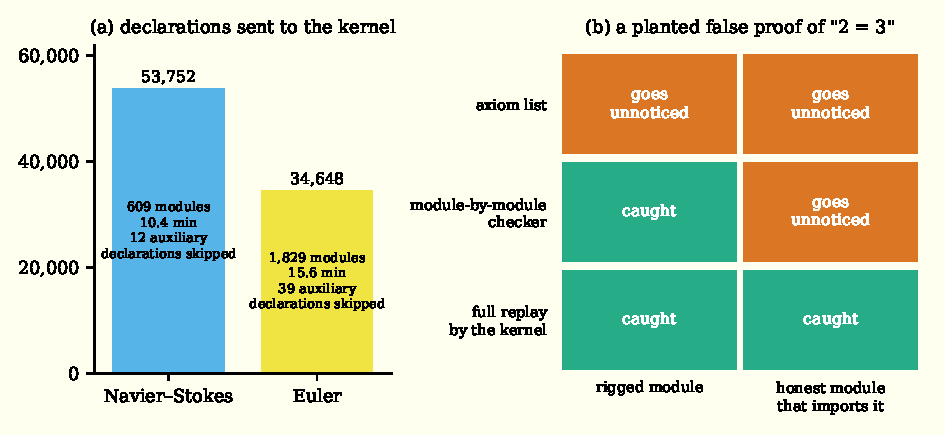
\includegraphics[width=\linewidth]{figures/c15_rejeu}
\caption{(a) Declarations sent back to the kernel, by corpus. (b) Only the full replay catches the false proof, even in an honest module that imports it.}
\end{figure}
